\documentclass[aps,twocolumn,showpacs,superscriptaddress]{revtex4}
%\documentclass[aps,showpacs,superscriptaddress]{revtex4}
\usepackage[pdftex]{graphicx}   % for figures
\usepackage{epstopdf}
%\usepackage{epsfig}
%draft
\usepackage{dcolumn}
\usepackage{bm}	
\usepackage{textcomp }
\usepackage{amsmath}			% Mode math\ufffdmatique
\usepackage{amsfonts}			% Polices math\ufffdmatiques
\usepackage{amssymb}			% Symboles math\ufffdmatiques
\usepackage{latexsym}			% Symboles math\ufffdmatiques avanc\ufffds
\usepackage{color}
\begin{document}

\title{Untangling resistive and collisionless electron filamentation instabilities in dense plasmas over large spatiotemporal scales}

\author{C. Ruyer}\email{charles.ruyer@cea.fr}
\affiliation{LULI - CNRS, Ecole Polytechnique, CEA : Universit\'e Paris-Saclay ; UPMC Univ Paris 06  : Sorbonne Universit\'es - F-91128 Palaiseau cedex, France}
\affiliation{SLAC National Accelerator Laboratory, Sand Hill Road, Menlo Park, California, USA}
\affiliation{CEA, DAM, DIF, F-91297 Arpajon, France}
\author{S. Bolanos }
\affiliation{LULI - CNRS, Ecole Polytechnique, CEA : Universit\'e Paris-Saclay ; UPMC Univ Paris 06  : Sorbonne Universit\'es - F-91128 Palaiseau cedex, France}
\author{B. Albertazzi}%\email{Bruno.albertazzi@polytechnique.edu}
\affiliation{LULI - CNRS, Ecole Polytechnique, CEA : Universit\'e Paris-Saclay ; UPMC Univ Paris 06  : Sorbonne Universit\'es - F-91128 Palaiseau cedex, France}
\affiliation{ INRS-EMT, Varennes, Qu\'ebec, Canada}
\author{S.N. Chen}
\affiliation{LULI - CNRS, Ecole Polytechnique, CEA : Universit\'e Paris-Saclay ; UPMC Univ Paris 06  : Sorbonne Universit\'es - F-91128 Palaiseau cedex, France}
\affiliation{Institute of Applied Physics, 46 Ulyanov Street, 603950 Nizhny Novgorod, Russia}
\author{P. Antici}
\affiliation{ INRS-EMT, Varennes, Qu\'ebec, Canada}
\author{J. B\"oker}
\affiliation{Institut f\"ur Laser-und Plasmaphysik, Heinrich-Heine-Universit\"at, D\"usseldorf, Germany}
\author{V. Dervieux}
\affiliation{LULI - CNRS, Ecole Polytechnique, CEA : Universit\'e Paris-Saclay ; UPMC Univ Paris 06  : Sorbonne Universit\'es - F-91128 Palaiseau cedex, France}
\affiliation{CEA, DAM, DIF, F-91297 Arpajon, France}
\author{ L. Lancia}
\affiliation{LULI - CNRS, Ecole Polytechnique, CEA : Universit\'e Paris-Saclay ; UPMC Univ Paris 06  : Sorbonne Universit\'es - F-91128 Palaiseau cedex, France}
\affiliation{Dept. SBAI, Universita di Roma ``La Sapienza'', Via A. Scarpa 14 00181 Rome, Italy}
\author{M. Nakatsutsumi}
\affiliation{LULI - CNRS, Ecole Polytechnique, CEA : Universit\'e Paris-Saclay ; UPMC Univ Paris 06  : Sorbonne Universit\'es - F-91128 Palaiseau cedex, France}
\author{L. Romagnani}
\affiliation{LULI - CNRS, Ecole Polytechnique, CEA : Universit\'e Paris-Saclay ; UPMC Univ Paris 06  : Sorbonne Universit\'es - F-91128 Palaiseau cedex, France}
\author{R. Shepherd}
\affiliation{LLNL, Livermore, United States}
\author{M. Swantusch}
\affiliation{Institut f\"ur Laser-und Plasmaphysik, Heinrich-Heine-Universit\"at, D\"usseldorf, Germany}
\author{M. Borghesi}
\affiliation{School Physics and Astronomy, The Queen's University, Belfast, United Kingdom}
\author{O. Willi}
\affiliation{Institut f\"ur Laser-und Plasmaphysik, Heinrich-Heine-Universit\"at, D\"usseldorf, Germany}
\author{H. P\'epin}
\affiliation{ INRS-EMT, Varennes, Qu\'ebec, Canada}
\author{M. Starodubtsev}
\affiliation{Institute of Applied Physics, 46 Ulyanov Street, 603950 Nizhny Novgorod, Russia}
\author{M. Grech}
\affiliation{LULI - CNRS, Ecole Polytechnique, CEA : Universit\'e Paris-Saclay ; UPMC Univ Paris 06  : Sorbonne Universit\'es - F-91128 Palaiseau cedex, France}
\author{C. Riconda}
\affiliation{LULI - CNRS, Ecole Polytechnique, CEA : Universit\'e Paris-Saclay ; UPMC Univ Paris 06  : Sorbonne Universit\'es - F-91128 Palaiseau cedex, France}
\author{L. Gremillet}\email{laurent.gremillet@cea.fr}
\affiliation{CEA, DAM, DIF, F-91297 Arpajon, France}
\author{J. Fuchs}\email{julien.fuchs@polytechnique.edu}
\affiliation{LULI - CNRS, Ecole Polytechnique, CEA : Universit\'e Paris-Saclay ; UPMC Univ Paris 06  : Sorbonne Universit\'es - F-91128 Palaiseau cedex, France}
\affiliation{Institute of Applied Physics, 46 Ulyanov Street, 603950 Nizhny Novgorod, Russia}

\begin{abstract}
Plasma micro-instabilities induced by high-energy particle currents play an important role in many space or laboratory plasma environments. Here, we report on measurements that reveal, over large temporal (tens of picoseconds) and spatial (hundreds of microns) scales, the growth of a multiplicity of magnetic filaments, following localized laser-generation of MeV electrons in a solid foil. The proton radiography data obtained in both  low- and high-resistivity targets show two distinct, superimposed magnetic-field patterns, which point to different field generation processes, namely of collisionless and resistive character. The collisionless Weibel  instability is suggested, by particle-in-cell simulations, to build up in the dilute plasma expanding into the vacuum, independently of the target material, and to lead to observed azimuthally symmetric magnetic structures. Additionally, when the target resistivity is high enough, an additional resistive filamentation instability arises through the bulk target, resulting in observed radially elongated filaments.
\end{abstract}
\maketitle

The interaction of high-energy, charged particle flows with plasmas is a fundamental question in plasma physics and, more generally, physical kinetics. The energy and momentum transfers between the plasma species are mediated by either Coulomb collisions \cite{Shkarofsky_1966} or collective processes \cite{Belmont_2013}, depending on the density and velocity distributions of the plasma populations. Collective processes often give way to plasma micro-instabilities, \emph{i.e.}, growing electrostatic or electromagnetic waves that develop at kinetic electron or ion scales in systems with multi-stream or anisotropic momentum distributions \cite{Davidson_1983, Gary_1993}. 

An important class of instabilities is the Weibel-type current filamentation instability, which originates from thermal anisotropy \cite{PRL_Weibel_1959} or relative drifts between the plasma species \cite{POF_Fried_1959}. It generates small-scale electromagnetic fluctuations, which tend to deflect and thermalize the interacting particles \cite{POF_Davidson_1972, PRL_Lee_1973, POP_Silva_2002, APJ_Jaroschek_2004, PRL_Adam_2006}. This mechanism is drawing strong interest in high-energy astrophysics as it is suspected to mediate the creation of collisionless shocks, and their related phenomena, in weakly magnetized (electron-ion or electron-positron) plasmas \cite{APJ_Medvedev_1999, RPP_Marcowith_2016}. It is also a possible mediating agent for magnetization of the intergalactic medium \cite{APJ_Schlickeiser_2003}.
%
Much effort is currently expended in designing experiments to investigate this instability in the laboratory, either using conventional accelerator beams \cite{PRL_Allen_2012}, or laser-generated beams \cite{PRL_Fox_2013,NP_Huntington_2015},
the latter being favored by many teams for the high-density, high-current beams that can be obtained, as well as for the variety of plasma conditions that can be simultaneously produced using auxiliary beams. 

In the case addressed here where ultraintense ($>10^{18}\,\rm W.cm^{-2}$) short ($\lesssim 1\,\rm ps$) laser pulses impinging onto overcritical targets are used to generate ultrahigh (MA) currents of energetic (MeV) electrons, the Weibel/filamentation instability spontaneously arises from the interpenetration of these fast electrons and the background plasma. Around the laser spot, the plasma is heated to very high temperatures, and hence the instability is mainly collisionless and builds up at electron kinetic scales \cite{PRL_Adam_2006}. As of now, experimental evidence for the resulting small-scale surface magnetic fields has been obtained through high-resolution polarigrams only \cite{PNAS_Mondal_2012}. Fast electrons, however, can be prone to further filamentation when propagating through the target bulk. The resistive character of the cold plasma electrons making up the fast-electron-neutralizing return current \cite{POP_Gremillet_2002} then leads to larger magnetic filaments \cite{JPP_Fiore_2010} and enhanced fast-electron scattering \cite{POP_Yang_2016}. 
Such resistive filamentation has been diagnosed either indirectly, from spatial modulations of the sheath-field-accelerated protons \cite{PRL_Fuchs_2003, PRL_McKenna_2011, PRL_MacLellan_2013}, or directly,
from the optical emission by the fast electrons  \cite{PRL_Jung_2005, PRL_Storm_2009}.
Finally, the collisionless Weibel instability can also arise from fast electrons interacting with micron-scale-length plasma gradients at the target surfaces \cite{PRE_Wei_2004, PRL_Gode_2017, NJP_Scott_2017}.

\begin{figure}[tbh!]
\centerline{
\begin{tabular}{c}
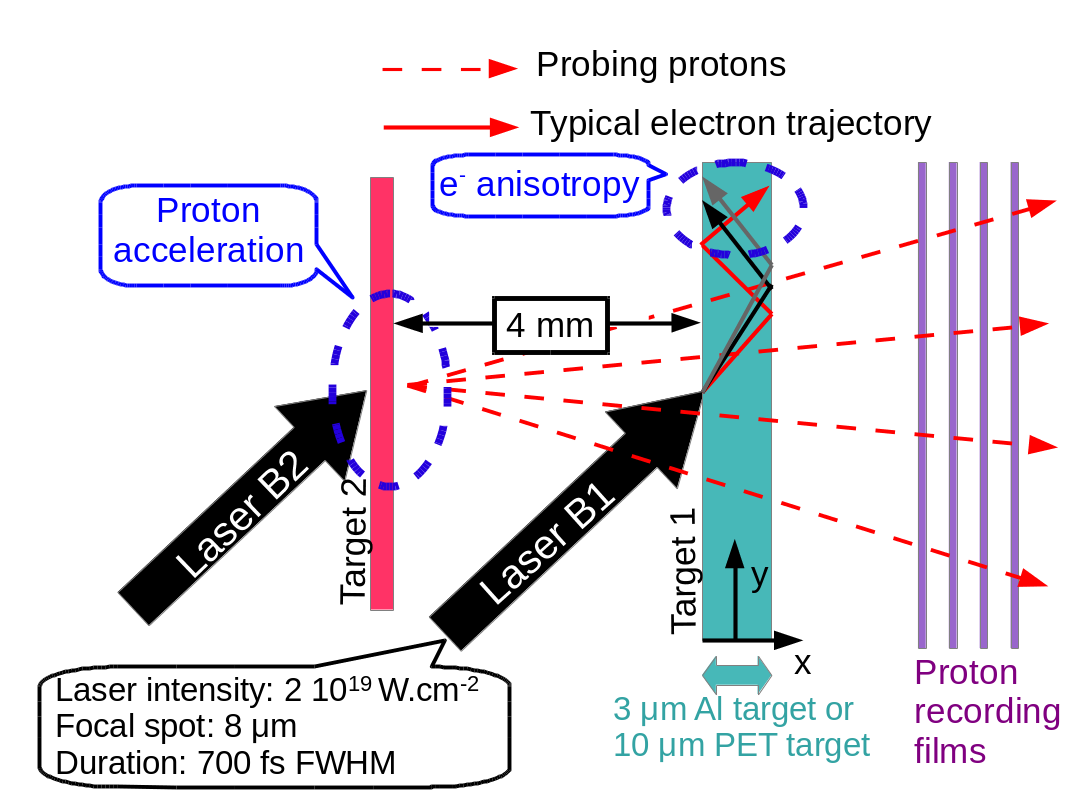
\includegraphics[scale=0.25]{sketch.png}\\
\end{tabular}}
\caption{\label{fig:xp} \textbf{Sketch of the experimental configuration and physical picture}. Target 1 is in red, target 2 in green.}
\end{figure}
The experimental and numerical data gathered so far seem to suggest that magnetic filaments only form relatively near the laser axis (over a few tens of microns), where the fast electron density, and therefore the overall plasma anisotropy, are initially at their highest. Furthermore, in contrast with simulation results \cite{POP_Heron_2015, POP_Yang_2016}, there has been as yet no observation of the simultaneous development of the collisionless and resistive variants of the instability in, respectively, the surface and inner regions of dense targets. 
Here we present measurements and simulations demonstrating: (1) filamentary magnetic-field generation by fast electrons over spatial (hundreds of microns) and temporal (tens of ps) scales much larger than previously thought possible; (2) the simultaneous development of the collisionless and resistive types of filamentation in different areas of the target, allowing us to untangle the conditions for their occurrence.

Our measurements are performed using a proton radiography technique \cite{LPB_Borghesi_2002}, under high-temporal contrast conditions \cite{RSI_Albertazzi_2015}. The setup employs two short-pulse laser beams, B1 and B2 (see Fig.~\ref{fig:xp} and Methods). B2 irradiates target 2 (a $3\,\rm \mu m$ thick Al or PET foil), while B1 generates the probe protons from target 1. Depending on target 2's material (Al being a conductor, PET being an insulator), two types of magnetic-field patterns are observed to arise, which kinetic simulations indicate are induced by the collisionless and resistive Weibel/filamentations instabilities. These are triggered as the fast electrons, respectively, recirculate in the low-density plasma expanding into the vacuum and drift away from the laser spot into the cold, solid-density target bulk. As will be detailed below in Figs.~\ref{fig:pic} and \ref{fig:kxy}, such instabilities give rise to magnetic structures consistent with the experimental results observed for both the Al and PET foils in terms of field strength, wavelength ($\sim 100\,\rm \mu m$), as well as spatiotemporal evolution (instability triggered a few $100\,\rm \mu m$ away from the focal spot, $\sim 4\,\rm ps$ after the main laser drive).
%
\begin{figure*}[tbh!]
\begin{tabular}{cc}
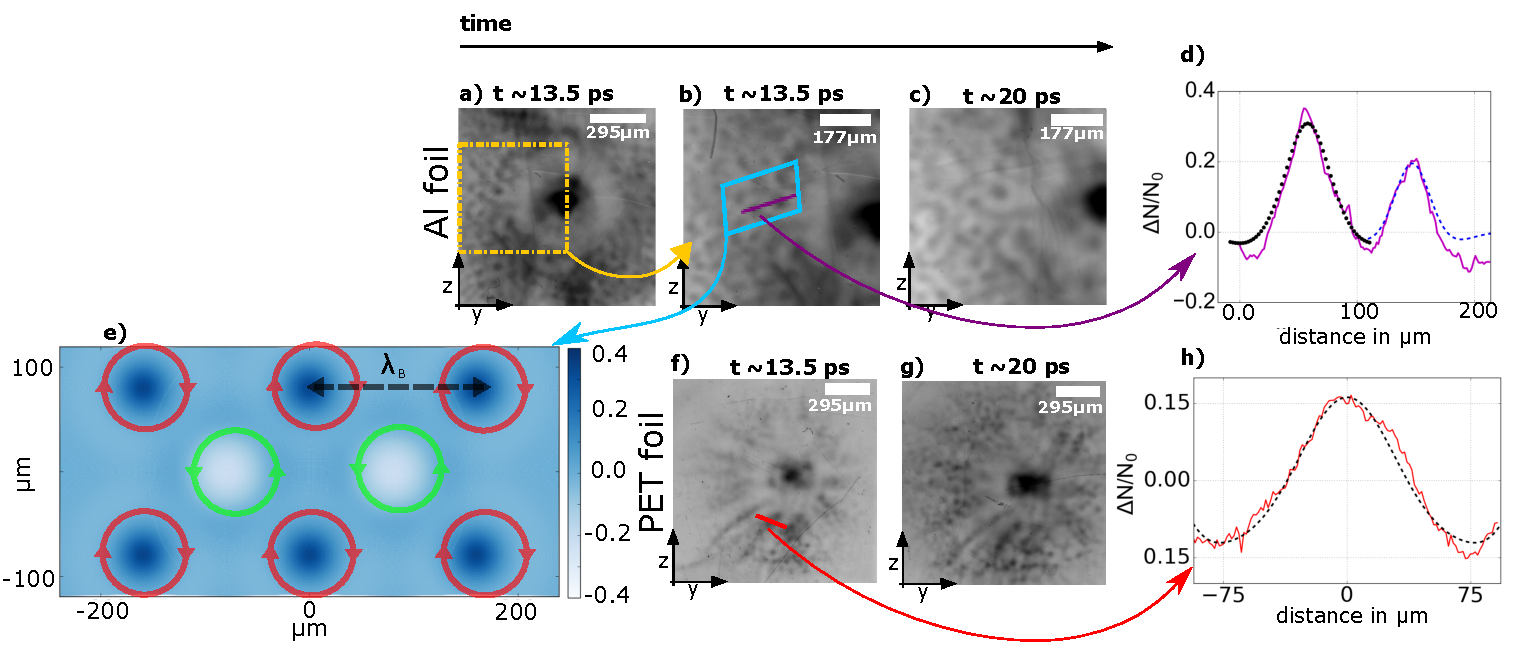
\includegraphics[scale = 0.6]{panel_v5.pdf}
\end{tabular}
 \caption{\label{fig:radio} 
\textcolor{red}{A mettre a jour, inclure le champs electrique dans e : comparaison B et B+E}
\textbf{Experimental proton radiographs evidencing two types of instabilities affecting hot electrons generated in solid foils, and the associated magnetic fields resulting from the electron filamentation, depending on the initial resistivity of the target.  }
(a-c) radiographs of Al as target 2, at various times ($t=0$ refers to the time at which laser B2 irradiates target 2). Darker and lighter areas correspond to increased and depleted proton dose, respectively \cite{RSI_Albertazzi_2015}. 
(b-c) Close-up view of an off-center region of the Al foil [delimited by the yellow dashed square in (a)]. 
Note that the small-scale filaments are observed to extend over the whole foil surface start to appear around $\sim 4\,\rm ps$ after laser irradiation.
(d) proton dose variation lineout corresponding to  the purple line  marked in (b). 
(e) cartoon of the postulated magnetic field topology (the loops with arrows marked in red and green) in the zone that is delimitated by the blue box in (b), and simulated proton dose modulation resulting from such magnetic field pattern. 
(f-g) proton radiographs obtained with target 2 being here a PET foil. On top of the small-scale circular filaments seen in (a-c), one observes here longitudinal proton dose streaks extending from the central laser-irradiation spot. 
(h) proton dose variation lineout corresponding to the red plain line marked in (f).
All frames, for either the Al or PET foil, corresponding to different energies of the probing protons, and hence to different times-of-flight between target 1 and target 2 (as indicated above each frame), are taken from a single shot. All spatial scales refer to the target 2 plane.
}
\end{figure*}

On the radiographs shown in Fig.~\ref{fig:radio}, B2 irradiates the foil with an angle of $31^\circ$ from the target normal, which corresponds to the laser pulse coming from the right of the images. 
As the dark and white region of the detector corresponds to probing proton accumulation and depletion respectively, 
the focal spot of B2 can be located by the large black area encircled by a white ring of $\sim 200\,\rm \mu m$ radius, delineating the large-scale $B$-field created by the Biermann battery on the surfaces of target 2 \cite{RSI_Albertazzi_2015} \textcolor{red}{and references therein}. Remarkably, the radiographs also evidence small-scale dark dots, appearing from $\sim 400$ to $\gtrsim 700\,\rm \mu m$ away from the focal spot. The typical wavelength of such modulations is $\lambda_B \sim 100\,\rm \mu m$ [see lineout in Fig.~\ref{fig:radio}(d)].
These structures, absent without B2 irradiating target 2 (the protons then exhibit a homogeneous dose, see Fig.~2(i) of Ref.~\cite{RSI_Albertazzi_2015}), are observed starting from $t=4-8\,\rm ps$. Note that proton dose fluctuations can be seen in an early time radiograph ($0-1\,\rm ps$, see first frame of Fig.~2(a) of Ref.~\cite{RSI_Albertazzi_2015}), although they do not then appear as fully formed loops. Additionally, they are preferentially located at the bottom left-hand side of the irradiated region, \emph{i.e.}, where the hot electrons are preferentially expected to be generated.
\textcolor{red}{Figure~\ref{fig:radio}(e) shows an idealized B-field loop-like topology (indicated by the arrows) and the influence of the electric field resulting from electron pressure (see Methods),
which results in black dots  consistent with the observations made with the radiographs.}  

The radiographs of the PET targets [Figs.~\ref{fig:radio}(f-g)] reveal a dotted pattern qualitatively similar to that seen in the Al foil. However, large-scale radial black streaks are superimposed to the previously observed circular structures. This suggests that another topology of B-field compared to the one shown in Fig.~\ref{fig:radio}(e), and which is not measurable for the case of the Al foil, is observed for the PET foil on the line of sight of the probing protons. 
We will now show that conditions are met, in the plasma  expanding from the target surface, and far from the focal spot, for the triggering of a collisionless Weibel-type instability due to the recirculation of the fast electrons, and leading to dark spot-type magnetic structures, such as the ones illustrated in Fig. \ref{fig:radio}(e). 
In order to investigate the hot electron dynamics on the required picosecond and millimeter scales, we have resorted to using 2D Particle-In-Cell (PIC) \textsc{calder} \cite{NF_Lefebvre_2003} simulations, resolving the laser plasma interaction in 2D geometry, in the same plane as shown in Fig.~\ref{fig:xp},  with reduced aluminum density (see Methods).
%
\begin{figure*}[tbh!]
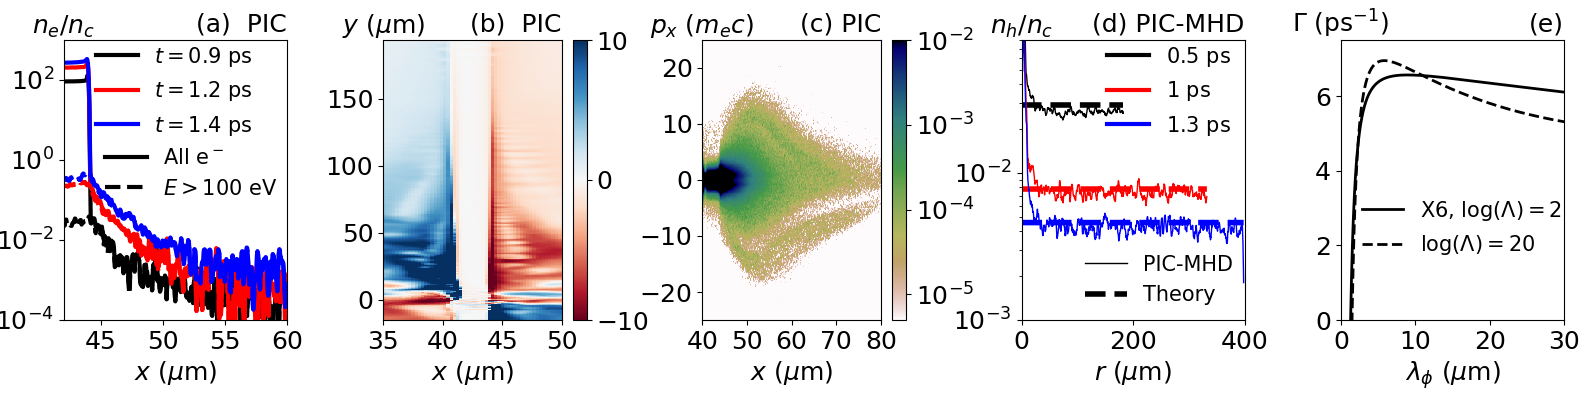
\includegraphics[scale=0.4]{figure_3.png}
\caption{\label{fig:pic} 
\textbf{Numerical simulations demonstrating the occurrence of plasma conditions favorable for the growth of the collisionless Weibel and the resistive filamentation instability. }
(a,b,c) Full 2D PIC simulation of  laser-plasma interaction in the plain (x,y).
(d) PIC-MHD simulation of hot electron thermalization in the plane (y,z).
(a)  Longitudinal lineout at $y=117\,\rm \mu m$ of the total (plain lines) and hot ($E\ge 100\,\rm eV$, dashed lines) electron density normalized to the laser critical density, illustrating the plasma expansion along the target normal and away from the laser irradiation spot (located at $y=0$).  
(b) Magnetic field   normalized to $1000\,\rm T$ at $t =1.44\,\rm ps$, illustrating the radial expansion of the hot electrons and the induced magnetic field as the result of the instability growth.
(c) Lineout at $y = 117\,\rm \mu m$ of the electron $(x,p_x)$-phase space for $E>100\,\rm eV$  at $t =1.44\,\rm ps$. 
%%%%%%%%%%%%
(d) Radial electron density profiles at different times  for the PIC-MHD simulation with $T_{h0} = 1\,\mathrm{MeV}$, $T_{c0} = 50\,\rm eV$, $n_{h0} = 5 \times 10^{21}\,\rm cm^{-3}$, $R_0 = 32\,\rm \mu m$ and $\log \Lambda =2$ as plain lines. The numerical results and analytical  estimates of $n_h$ (see text) are in thin plain lines and thick dashed lines respectively.
(e) Growth  rate of the instability (in $\rm ps^{-1}$) from the  resistive dispersion relations as a function of the poloidal wavelength (see Supplemenary Information) solved for the hot electron parameters extracted from the PIC-MHD simulations shown in (d) at $0.\,\rm ps$ ($n_h \simeq 2\times 10^{19}\,\rm cm^{-3}$,  $T_{x} \simeq 300\,\rm keV$, $T_{ec} \simeq 500\,\rm eV$, $v_r=0$,  $T_\phi = 10\,\rm keV$ and $13\,\rm keV$ for plain  and dashed line respectively, see method). 
The plain and dashed lines corresponds to $\log(\Lambda)=2$ (\emph{i.e.} representing a conductor, growth rate value multiplied by six) and $20$ (\emph{i.e.} representing an insulator). 
}
\end{figure*}
We see in Fig.~\ref{fig:pic}(a) that, already after $1.44\,\rm ps$ of laser plasma interaction, and at least $100\,\rm \mu m$ away from the laser focal spot, the target is longitudinally  expanding, and that  a magnetic modulation  of wavelength, $\lambda_p \sim 6\,\rm\mu m$ is observed [see Fig.~\ref{fig:pic}(b), around $0\,\rm \mu m$ $<y<150\,\rm \mu m$ and $x>44\,\rm \mu m$, and lineout in Figs.~S7(a,b) in Supplementary Information.
 Note that the magnetic field  pointed out in Ref.~\cite{PRL_Gode_2017} is consistent with what is observed in our  experimental radiographs in term of circular topology, but with a much larger  amplitude. 
 The electron phase space in the vicinity of the magnetic filaments at $y = 117\,\rm \mu m$ [see Fig.~\ref{fig:pic}(c)] evidences the superposition of the expanding hot electrons [for  $y > 300c/\omega_0$ of momentum $\vert p_x \vert \lesssim 10 m_ec$] with an electron return current for $-20 m_ec < p_x< -10\,\rm m_e c$.
According to Refs.~\cite{POP_Ren_2006, PRL_Gode_2017}, %NJP_Scott_2017},
this configuration  is unstable to Weibel-type instabilities with a maximum growth rate obtained for equal hot-electron and background plasma electron densities. Moreover, the magnetic-field wavelength and strength are related to the hot electrons plasma frequency [$\omega_{ph}=(n_h e^2/m_e \epsilon_0)^{1/2}$] through 
\begin{align}
 \lambda_p &\sim  2\pi c/\omega_{ph} \label{eq:lp}  \, ,\\
 B_p       &\sim m_e \omega_{ph}/(e2\pi) \label{eq:bp} \, , 
\end{align}
where $c$, $\epsilon_0$, $n_h$, $m_e$ and $e$  are the speed of light in vacuum, the permittivity in vacuum,  the hot electron density, the electron mass and  charge respectively.
\textcolor{red}{
Additionally, a radial electric field resulting from a charge imbalance between the magnetically pinched electrons and the ions in the vicinity of the filament is to be accounted, verifying 
\begin{align}
E_p \sim m_ec\omega_{ph} /(4\pi^2\gamma_h^{3/2} e) \label{eq:ep} \, .
\end{align}
Finally, the expected magnetic field loops of alternative polarity are  focusing or defocusing for the probing protons according to the filament's current sign. This contrasts with the electric field  topology, which is always focusing and  can contributes to  the resulting radiograph [see Fig.~\ref{fig:radio}(e) and Fig. S... of the Supplemental Material].
}

In order to relate the magnetic-field wavelength observed on the aluminum radiographs and th observed  in the simulation as in Fig. \ref{fig:pic}(b), and thus verify if the instability observed is indeed leading to the magnetic loops experimentally observed in Fig.~\ref{fig:radio} (dark spot in the radiographs), we have to analytically disentangle the impact of the  reduced-geometry of our simulation on the hot electron dynamics. 
Indeed, unlike in Refs. \cite{PRL_Gode_2017,NJP_Scott_2017}, we observe [see Fig.~\ref{fig:radio}(b)] fields hundreds of microns away from the focal spot, and at least a picosecond after the laser irradiation, implying that late time multi-dimensional hot-electron dilution is to be expected. 
However, the radial particle spreading inside  the foil plane is obviously missing in our 2D full-PIC simulation [Fig.~\ref{fig:pic}(a-c)] since it treats only of the (x,y) plane. The effect of the 3D geometry on the hot-electron dynamics will thus be evaluated by estimating by the   temporal evolution  of $n_h$ in a general system of dimension $D+\delta$ where $D$ and $\delta$ are the number of dimensions in the target plane and normally to it, respectively.
Assuming an homogeneous distribution over the hot electron light cone, the hot electron density thus reads $n_{h}\sim n_{h,  t=0} /(1+ v_h t /R_0)^D/(1+c_s t/L)^\delta $ with $t$, $L$, $c_s$ and $R_0$ being the time, target thickness, hot-electron sound speed and initial electron deposition radius (see Supplementary Information). 
This estimate remains valid far from the irradiated region after the laser has deposited its energy and  a good agreement is illustrated in Fig.~\ref{fig:pic}(d)   with dedicated PIC-MHD 2D simulations of hot electrons, implemented into the code \textsc{calder} (see Methods), and performed this time in the target plane ($D=2$, $\delta=0$).
The 2D PIC-MHD simulations allow us to study the main collective and collisional processes ruling the large-scale hot electron expansion by treating the response of the thermal target electrons in the resistive MHD limit (see Methods). More precisely, our reduced model describes the 2D (y,z) dynamics of a population of hot electrons of temperature $T_{h0}=1 \,\rm MeV$, initially localized in a circular region of radius $R_0=32\,\rm \mu m$, and spreading within a solid-density, collisional Al plasma. 
Care has been taken to verify that these initial hot electron parameters are consistent with the results of our 2D laser-plasma fully PIC simulation (see supplemental material). Finally, the target electron temperature is initialized at $50\,\rm eV$ in order to remain in  the regime of validity of the PIC-MHD framework that  fails to capture the solid  density physics below a few $10\,\rm eV$ \cite{POP_Perez_2012}. Moreover, the PIC-MHD simulations allow us to model the system over longer times scales that the fully kinetic simulation, which is limited to the picosecond timescale, short in comparison with the experimental observations.
%
%%%%%%%%%%%%%%%%%%%%%%%%%%%%%%%%%%%%%%%%%%%%%%%%%
At  $t = 1.4\,\rm ps$, the laser-plasma interaction simulation presents a hot electron profile that peaks at $n_{h, t=0} \sim 5\times 10^{21}\,\rm cm^{-3}$ and extends over a distance $R_0\sim 32\,\rm \mu m$ (see Supplementary Information), giving, for $D=\delta=1$, $n_h \sim 8 \times 10^{19}\,\rm cm^{-3}$.
Making use of Eqs.~\eqref{eq:lp}, \eqref{eq:bp} and \eqref{eq:ep}, we obtain $\lambda_p \sim 4 \,\rm \mu m$, $B_p \sim 509\,\rm T$ and $E_p\sim 24\,\rm GV.m^{-1}$ in fair agreement with the simulation, as can be inferred from Fig.~\ref{fig:pic}(b) and Fig.~S7(a) in Supplementary Information. 
\textcolor{red}{
In the experiment ($D=2$, $\delta=1$) for which the time of first experimental observation is $\sim 4$ ps, we obtain
$\lambda_p \sim 58 \,\rm \mu m$ which is consistent with the size of the structures observed in Fig.~\ref{fig:radio}(a-c), and   $B_p\sim 24\,\rm T$, also comparable with the experimental estimates of $\sim 10\,\rm T$ (see section method). As for the electric field amplitude, we obtain $E_p \sim 1.5\,\rm GV.m^{-1}$ which is enough for affecting  the radiographs as shown in Fig.~\ref{fig:radio}(e) (see Supplementary Information...).
}

The  2D PIC-MHD simulation lying in the target plane, therefore neglecting the expansion direction, also allows us to address the radial spreading dynamics of the hot electrons and the subsequent resistive instability that can affect them. As the electrons move radially away from their generation region into the dense foil, their momentum distribution becomes ``cold'' in the poloidal direction, while it stays ``hot'' along the other directions (see Fig.~5 in Supplementary Information). A large hot electron pressure anisotropy is therefore driven in $\sim 0.5\,\rm ps$ in our 2D PIC-MHD simulation, although its final amount may be overestimated due to the target expansion in the $x$-direction (and the associated electron-to-ion momentum-transfer which should occur in $\sim L/2c_s \sim 0.5\,\rm ps$ \cite{PRE_Mora_2005}, \textcolor{red}{see Supplementary Information}), neglected in our 2D PIC-MHD simulation. 
\begin{figure*}
\centerline{
\begin{tabular}{ccc}
(a) PIC-MHD Magnetic field  &  (b) Resulting radiograph &  (c) With expanded plasma contribution\\
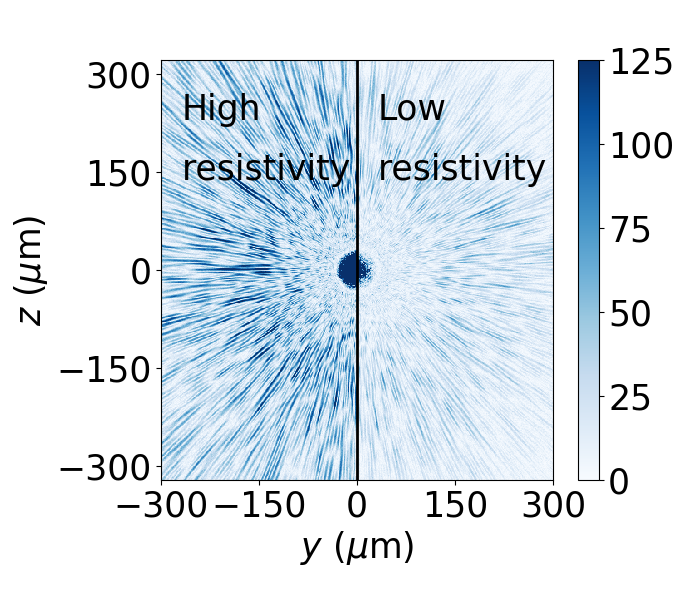
\includegraphics[scale=0.33]{B_Te0_05_ne300_nh5_Th1MeV_t10500_complog.png} &
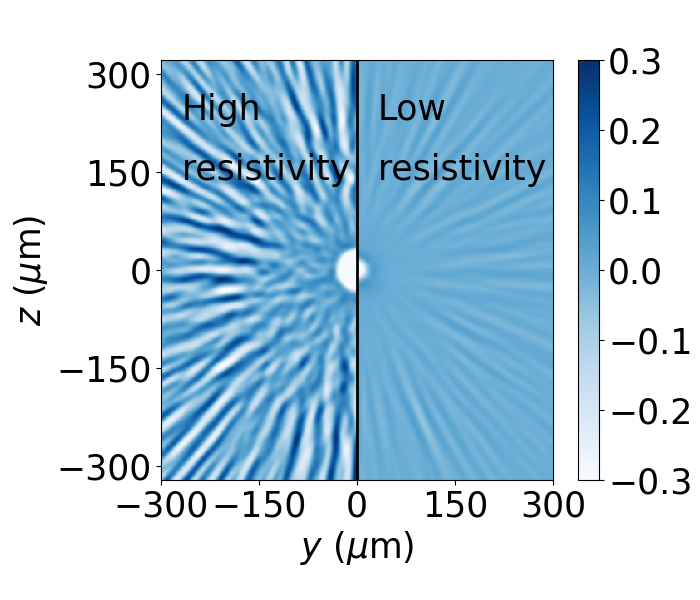
\includegraphics[width=0.33\textwidth]{DN_Te0_05_ne300_nh5_Th1MeV_t10500_complog_300mum.png} &
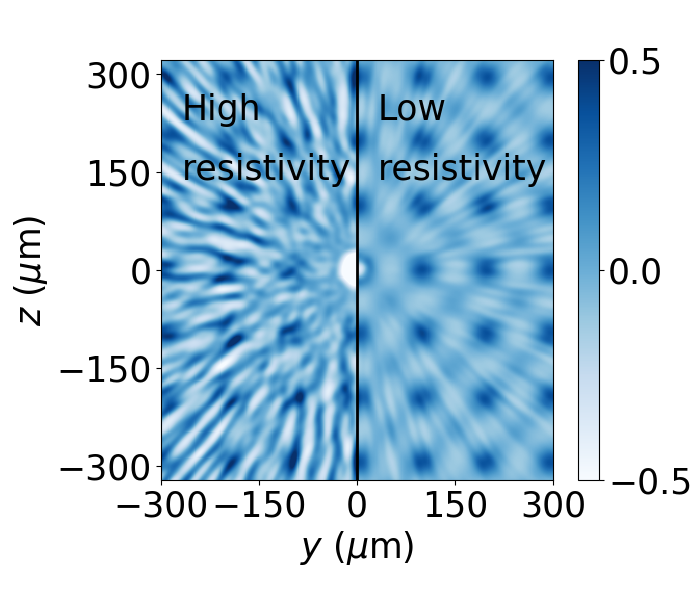
\includegraphics[width=0.33\textwidth]{DN3D_complog_R20_a60_l140.png}
\end{tabular}}
\caption{\label{fig:kxy} 
\textbf{2D PIC-MHD simulations evaluating the growth of the resistive filamentation in the solid foil plane for various initial resistivity values.}
(a) Magnitude of $B_\perp=(B_x^2+B_y^2)^{1/2}$ (in Teslas) at time $t=3.28\,\rm ps$ for $\log \Lambda=20$ (\emph{i.e.} modeling an insulator, $y<0$) and $\log\Lambda=2$ (\emph{i.e.}, modeling a conductor, $y>0$).
(b) Simulated radiographs from 8 MeV probing protons in a 
$3\,\rm \mu m$ thick target with B-fields given by (a), see method.
(c) Modeled radiographs with superimposed filaments extending in the z direction over $L_p = 48\, \mu$m, see method. The $B$ field profile used for the reconstruction is poloidal around of the each filament center following Fig. \ref{fig:radio}(e) with $\lambda_B = 120\,\rm \mu m$, and with a radial profile given by Eq. \eqref{eq:bloop} with $B_0=10\,\rm T$ and $a = 60\,\rm \mu m$.
}
\end{figure*}
%
As a consequence, in the case of a conductor modeled by using a Coulomb logarithm of $\log \Lambda = 2$,  a non-propagating magnetic modulation builds up after a few $100\,\rm fs$ [see \mbox{Fig.~\ref{fig:kxy}(a), right}], reaching a strength of  $\langle B_\phi^2\rangle^{1/2}\sim 34\,\rm T$ (where $\langle X \rangle$ is the spatial average of $X$ over the region  $100\,\mu\mathrm{m}<r<200\,\mu \rm m$) and a typical wavelength of $\sim 5-10\,\rm \mu m$  in the poloidal direction. The resistive dispersion relation, derived for the plasma parameter extracted from the PIC-MHD simulation at $0.5\,\rm ps$ and illustrated in Fig.~\ref{fig:pic}(e)  shows that the fastest growing mode verifies $\lambda_\phi \sim 5\,\mu \rm m$  in agreement with our simulation results. The instability  growth time, $\Gamma_\phi^{-1} \sim 160\,\rm fs$  is also  consistent with the first experimental manifestation of proton modulations appearing at $0-1\,\rm ps$ after laser irradiation.

We will now evaluate the influence of the target resistivity on the observed radial structures.
References \cite{PRL_McKenna_2011, PRL_MacLellan_2013} demonstrates the dependence of the fast electron current spatial distribution  on the resistivity in the few-eV range inside the solid. Hence, the fast electrons dynamics in the insulator PET target is expected to differ from the Aluminum's due to an increased resistivity at low temperature. In particular below $50\,\rm eV$, our PIC-MHD framework fails to be predictive so that we will restrict ourselves to a qualitative comparison by performing the same PIC-MHD simulation than in aluminum but with an artificially  increased resistivity, \emph{i.e.}, using  a Coulomb logarithm of $20$ instead of $2$, in order to attempt to mimic the PET target. The associated growth rate [dashed line in Fig.~\ref{fig:pic}(e)] is $\sim 6$ times larger than at low resistivity with  an  essentially unchanged dominant wavelength. This suggests \cite{POF_Davidson_1972} that the magnetic fields at saturation is larger for $\log\Lambda = 20$ than for $2$, which is confirmed by our numerical results illustrated in  the left side of Fig.~\ref{fig:kxy}(a) where  $\langle B_\phi^2 \rangle^{1/2} \sim 69\,\rm T$, twice larger  in amplitude than at low resistivity.

After saturation of  the resistive filamentation, the hot electrons current contribution vanishes due to dilution, so that the B-field structures are solely carried by the cold electron population and evolve due to magnetic diffusion  over a  timescale $\sim \mu_0 \sigma \lambda_\phi^2 > 30\,\rm ps$ for $ \ge 50\,\rm eV$ targets, consistently with experimental observations. This is why, although the latest time of the PIC-MHD simulation ($3.28\,\rm ps$) is still early in comparison to what is probed in the experiment,  we do not expect significant evolution of the fields inside the target over a few $10\,\rm ps$.

Hence, the proton synthetic radiographs, shown in Fig.~\ref{fig:kxy}(b,c), making use of the fields resulting from our PIC-MHD simulations, should be qualitatively representative of the expected radiographs (see method). Indeed,  large radial structures similar with the one observed experimentally for the PET target [see Figs.~\ref{fig:radio}(d,e)],  are obtained with increased  proton dose variation for increased resistivity. Note that the scattering of the probing protons off the aluminum dense foil ions have been accounted for (see Methods and Supplementary Information) and is mainly responsible of the smoothed rendering of Fig.~\ref{fig:kxy}(b) compared to \ref{fig:kxy}(a).
 %
Fig. \ref{fig:kxy}(c) corresponds to proton ray tracing simulations where the fields resulting from the PIC-MHD simulations has been juxtaposed to the field expected in the expanding plasma using circular field lines (see method). 
Overall, Fig.~\ref{fig:kxy} shows that at low resistivity, the expanding plasma contribution is dominant over the resistive traces, corresponding qualitatively to the aluminum radiographs of Figs.~\ref{fig:radio}(a,b). However, for larger resistivity, as in the PET target [Figs.~\ref{fig:radio}(c,d,e)], both the resistive and collisionless instability  contributions can be characterized experimentally  leading to strong constrains on the various field contributions (see Methods and Supplementary Information).
\textcolor{red}{
The lower number of radial structures observed in Fig.~\ref{fig:radio}(f) compared to   Fig. \ref{fig:kxy}(b) can be attributed to the strong uncertainty that remains on the initial hot electron parameters. The dominant magnetic wavelength of the resistive filamentation depends on the initial hot electron density which is   strongly dependent on the target properties at  early times where   solid state or strongly coupled plasma physics is at stake \cite{}. 
 }
 
The full quantitative understanding of the experimental results involves late time (tens of ps) and very large scale (hundreds of microns) hot electron kinetic physics in dense plasma  with important three dimensional  effects such as fast particle streaming and recirculation in an expanding target.
Not only numerically out of reach of the present or near-future largest available super-computers, the  underlying physics requires, still active area of research modeling, as the coupled-to-weakly-coupled plasma transition during laser irradiation  and self-generated electromagnetic fields and associated non-linear effects.
This experiment therefore highlights the importance of the science triptych:  experiment, simulation, theoretical modeling, in order  to tackle the formidable challenge of the  full understanding of kinetic effects affecting fast electrons in collisional and collisionless plasmas.


\section*{Methods}
\subsection*{Experiment}
The experiment %aimed at studying the long-time evolution of the laser-accelerated fast electrons into a solid,
was performed at the Jupiter Laser Facility's \textsc{titan} laser at the Lawrence Livermore National Laboratory \cite{RSI_Albertazzi_2015}. Each laser beam B1 and B2 \textcolor{red}{had an angle with the targets normal of 31$^O$}, an energy of $55\,\rm J$ $(\pm 10$\%$)$, a pulse duration of $\sim 700\,\rm fs$ FWHM and was focused with a $f/3$ parabola, resulting in an on-target intensity of $\sim 2\times 10^{19}\,\rm W.cm^{-2}$. Before focusing, B2 was reflected off a plasma mirror, with $70\,\%$ efficiency, in order to improve its temporal contrast \cite{PRE_Doumy_2004}. 
A high temporal contrast ensures steep density gradients at the target surface, which is critical (e.g. compare with the results of Ref.~\cite{PRL_Sarri_2012} where no similar far-distant filaments can be observed, likely due to the formation of a large preplasma on the target surface induced by the laser prepulse) for the formation and observation of the far-distant magnetic loop structures revealed here. The normalized laser-wave amplitude is $A_0 = eE/m_ec\omega_0 \simeq 4$, where $\omega_0$ is the laser frequency. Under our high-temporal-contrast and oblique-incidence conditions, hot electron generation is expected to be dominated by the so-called ``vacuum heating'' mechanism \cite{PRL_Brunel_1987}. After $700\,\rm fs$, when the laser-intensity drops, a significant fraction ($\sim 50\,\%$ \cite{PRL_Ping_2008}) of the $\sim 55\, \rm J$ laser energy has been converted into a total number of $\sim 10^{14}$ hot electrons.

The probing proton beam, generated through target normal sheath acceleration \cite{RMP_Macchi_2013} by focusing B1 onto a $50\,\rm \mu m$-thick Au foil, has a useful energy range of $4.5\,\rm MeV$ to $9.5\,\rm MeV$. It is used to probe the $B$-fields developing in target 2 in a ``face-on'' configuration \cite{RSI_Albertazzi_2015} adapted to probing toroidal magnetic loops having their axis along the target normal and to minimize the influence of the E-fields that develop along the target normal. As shown in Fig.~\ref{fig:xp}, the probing proton beam, after propagation through target 2, was collected by a stack of radiochromic films in which protons are stopped in different layers according to their incident energy. The difference in the time-of-flight of protons having different energies from their source up to target 2 allowed us to probe the central, large-scale, as well as the radially far, small-scale, $B$-fields at different times ($t=0$ corresponds to the time at which B2 strikes target 2).
Target 2 was either an Aluminium (Al) foil, being $3\,\rm \mu m$-thick, or a Polyethylene terephthalate [PET, an insulator polymer with composition $(\mathrm{C}_{10}\mathrm{H}_8\mathrm{O}_4)_n$], being $10\,\rm \mu m$-thick.
 
\subsection*{2D laser-plasma PIC simulation}

A large scale PIC simulation of the irradiation of the aluminum foil by a high intensity target with the PIC code \textsc{calder} has been performed.
The laser of maximum intensity of $3.5 \times 10^{19}\,\rm W.cm^{-2}$ reached at $1.03\,\rm ps$ the left hand simulation boundary. It had a Gaussian temporal profile with a FWHM (full width at half maximum) of $690\,\rm fs$,  a Gaussian spatial profile of $8\,\rm \mu m$ FWHM and a $30^\circ$ incident angle. The target is composed of three layers: neutral hydrogen ($0.7\,\rm \mu m$), Al$^{3+}$ ($3.7\,\rm \mu m$) and neutral hydrogen ($6\,\rm nm$) with a flat density profile of $3 \mu$m preceded by a $1.4\,\rm \mu m$-long preplasma made of H$^{0+}$ and Al$^{3+}$ ions. All species are initialized with a temperature of $10\,\rm eV$ and, in order to reduce the computational load, half of the maximum target density has been reduced by a factor two: $n_\mathrm{H} = n_{\mathrm{Al}^{3+}}90 n_c$.

The simulation domain is $L_x\times L_y = 48 \times 278\,\rm \mu m^2$ with a spatial discretization $\Delta x = \Delta y = 5.6\,\rm nm$ and a time step
$1.48\times 10^{-2}\,\rm fs$. We employ an alternating-order interpolation scheme \cite{CPC_Sokolov_2013} with a 4th-order weight factor. Each cells initially contains
50 macro-particles per species in the Al layer \textcolor{red}{and 500 macro-particles per species in the thin H layers}. Elastic Coulomb collisions, electron impact
ionization and field ionization are modeled following Refs.~\cite{POP_Nuter_2011, POP_Perez_2012}. Furthermore, we use the Maxwell solver proposed in Ref.~\cite{PRSTAB_Lehe_2013}, along with a combination of spatial \cite{JCP_Vay_2011} and temporal \cite{JCP_Friedman_1990} filtering.

\subsection*{2D PIC-MHD simulations}

In order to access spatio-temporal scales of experimental relevance in a 2D geometry, we have employed the resistive magnetohydrodynamic PIC model proposed in
\mbox{Ref.~\cite{JCP_Cohen_2010}}. This numerical scheme, implemented into the code \textsc{calder} \cite{NF_Lefebvre_2003}, consists in replacing the Maxwell-Amp\`ere equation
by the generalized Ohm's law
\begin{equation} \label{eq:PICMHD}
  \mathbf{E}=\eta \left(\nabla \times \mathbf{B}-\mathbf{J}_{h}-\frac{\partial \mathbf{E}}{\partial t}\right)+\frac{\mathbf{J}_{ec}\times \mathbf{B}}{en_{ec}}
  -\frac{\nabla P_{ec}}{en_{ec}} \,,
\end{equation}
where $\eta$ is the electrical resistivity, $n_{ec}$, $P_{ec}$ and $\mathbf{J}_{ec}$ are the density, pressure and current density of the thermal (`cold') electrons and $\mathbf{J}_h$ is the current density of the hot electrons. Since this scheme only accounts for the generation of non-radiative fields, it allows one to use mesh sizes (resp. time steps) much larger than the plasma skin depth (resp. plasma period), thus greatly alleviating the computational load. In a given cell, electrons are considered `cold' if their velocity fulfills $v<5\sqrt{T_{ec}/m_e}$, where $T_{ec}$ is the local temperature of the cold electron population
at the previous time step; the remaining electrons are considered `fast'.

Our PIC-MHD simulation, 2D in space and 3D in momentum, self-consistently describes the evolution of an initially confined source of hot electrons through a dense Al plasma in the $yz$ plane parallel to the target surface (assuming invariance along the $z$ axis). Initially, the hot electrons uniformly fill a cylinder of
$R_{0}$=$32\,\rm \mu m$ radius and $n_{h,t=0}$=$5n_c$ density, centered around $(y,z)=(0,0)$. The choice of an initial hot electron spot wider than the $\sim 8\,\mu\mathrm{m}$ laser spot partly accounts for the radial expansion of the hot electrons during the laser duration \cite{PRE_Stephens_2004} (thus ensuring a relatively moderate $n_{h,t=0}$, as is expected). Their momenta are distributed according to an isotropic Maxwell-J\"uttner distribution of temperature $T_{h0}=1\,\rm MeV$. Simulations performed with different initial temperatures (from $200$ to $500\,\rm keV$) or anisotropic distributions (with $T_x>T_{y,z}$) yield qualitatively similar results. The total kinetic energy carried by the hot electrons is $\sim 25\,\mathrm{J}$, which amounts to $\sim 50\%$ of the B2 laser energy \cite{PRL_Ping_2008}. The hot electron spot is immersed inside a solid-density Al$^{5+}$ plasma of \mbox{50-eV} temperature. The bulk electron density is $n_{ec,t=0}=300n_c$ everywhere, except within the hot spot, where it reduces to $295n_c$ to ensure charge neutrality. Coulomb binary collisions between all the charged particle species and impact ionization of the Al ions are described using the framework of \mbox{Ref.~\cite{POP_Perez_2012}}. The electrical resistivity involved in Ohm's law is calculated in the Spitzer regime with the numerical fits given in Ref. \cite{Decoster_1998}. 

Perfect electrostatic confinement of the hot electrons within the target is assumed and the effects of ion expansion into vacuum are neglected, particularly the energy losses suffered by the hot electrons driving this expansion \cite{POP_Antici_2013}; this is justified as the electrons quickly escape the laser-irradiated zone and since, in the cold plasma zones where the electrons propagate, these energy losses are minimal over the time scales discussed here \cite{PRL_Mora_2009}. 

The computational domain has dimensions
$L_x\times L_y=800 \times 800\,\rm \mu m^2$ and is discretized with mesh sizes $\Delta x=\Delta y =0.16\,\rm \mu m$. The time step is $\Delta t=0.34\,\rm fs$. The boundary conditions are taken to be absorbing for the particles and reflective for the fields. The ion and cold electron populations are initially modeled by 100 macroparticles per cell, while the hot electrons are modeled by 1000 macroparticles per cell.

\subsection*{ Resistive dispersion relation}
The electromagnetic dispersion relation of a homogeneous and resistive plasma in the presence of a hot-electron population has been derived. 
Assuming the ions at rest,  the hot electron current contribution is obtained by linearizing the Vlasov-Maxwell equations, while the cold electrons  of the target bulk are assume to fulfill a generalized Ohm's law, therefore enabling a kinetic description of the fast particle streaming into a resistive medium.
The  hot electrons are described by a  multi-Maxwellian distribution, neglecting the relativistic effects.
After a lengthy algebra and  a third-order Taylor development of the plasma dispersion, one obtains the linear growth rate as a function of the magnetic-fluctuation wavevetor and of the hot and resistive electrons parameters  (see Supplementary Information).
In order to compare the growth of the resistive instability in each PIC-MHD simulation, \emph{i.e.} corresponding to a conductor  [using $\log \Lambda=2$] and  an insulator medium [using $\log \Lambda=20$], we  extracted the plasma parameters from each simulation. 
in the case $\log \Lambda=2$, [Fig. \ref{fig:kxy}(a), right], the radial drift  poloidal temperature and $x$-aligned temperature at $t=0.5\,\rm ps$ reads
$T_\theta \simeq 10\,\rm keV$ and 
$T_x \sim 300$ keV, respectively, with $n_h\simeq 0.02 \times 10^{21}\,\rm cm^{-3}$ (see the dashed black lines of Figs.~5(a-e) in Supplementary Information). The case with $\log \Lambda =20$, [Fig.~\ref{fig:kxy}(a), left] gives $T_\theta \simeq 13\,\rm keV$,
$T_x \sim 300\,\rm keV$ and $n_h\simeq 0.02 \times 10^{21}\,\rm cm^{-3}$. 

The resistive electron temperature at $t=0.5\,\rm ps$ varies between $150\,\rm keV <T_{ec} < 600\,\rm keV$ [see Fig.~6(b) in Supplementary Information] and the radial drift velocity along $0< \vert v_r \vert <2\times 10^8 \,\rm m.s^{-1}$ [see Fig.~5(c)]. 
In the calculation of Fig. \ref{fig:pic}(e), use has been made of $T_{ec}=500\,\rm eV$ and $v_r = 0$.
Care has been taken to verify that both increasing $v_r$ up to $2\times 10^8 \,\rm m.s^{-1}$ and decreasing $T_{ec}$ to $150\,\rm eV$ increases the growth rate and does not change the qualitative ordering of the ``resistive'' and ``insulator''-type growth rates [plain and dashed lines of Fig.~\ref{fig:pic}(e)], thus remaining consistent with the experimental observations.

\subsection*{Synthetic radiographs \textcolor{red}{updates necessaires ici}}
The synthetic proton images and proton dose modulations presented in this paper (Fig.~\ref{fig:radio} and  \ref{fig:kxy}) have been made with the \textsc{ilz} numerical tool developed at LULI \cite{PHD_Riquier}. This synthetic proton radiography tool is used to compare qualitatively the 2D PIC simulations to the experimental results shown in Fig.~\ref{fig:radio}, and evaluate the topology of the magnetic fields inducing the experimental proton radiography analysis, as shown in Fig.~\ref{fig:kxy}.
\textsc{ilz} simulates the propagation of any kind of ion in a given electromagnetic field. Each ion trajectory is computed independently so that collective effects are neglected. This assumption is based on the very high laminarity of the laser-accelerated protons \cite{PRL_Cowan_2004} (here through the TNSA mechanism \cite{RMP_Macchi_2013}), meaning that the proton source size is very small ($\mu$m-scale) and that there is no proton trajectory crossing. The electromagnetic  fields   initialized by the user, are interpolated at the 0th up to the 2nd order and assumed static, which is reasonable regarding the short time-scale of the proton crossing time through the plasma ($0.15\,\rm ps$, since the protons are of several MeV energy for the proton radiography presented in this paper) with respect to the typical magnetic field time-scale ($\sim 0.5\,\rm ns$, as given by the Alfven velocity). The charged particle motion through the electromagnetic  field structure is resolved with the Boris “leap frog” algorithm, which conserves the energy. In all of these simulations the incident proton flux has been initialized angularly uniform and monochromatic. Then the code reconstruct the dose variation onto the detector plane, $\Delta N/N_0= (N- N_0)/N_0$ with $N$ the local (in a given solid angle) quantity of ions deflected by the fields and $N_0$ the quantity prior the ion crossing  (in the same solid angle). 
The loss of energy and the scattering of the ions through the matter have not been implemented in the code. Regarding the first, since the plasma is thin, for MeV protons, the energy loss is indeed negligible. Regarding their scattering, it will be mostly induced by passing through the solid-density material of the target substrate. To model it, \emph{i.e.}, in order to mock-up the Moliere's scattering of protons through the foil of aluminum or PET \cite{Moliere_1947}, we convolve the dose variation calculated by \textsc{ilz} in the detector plane with a Gaussian function which represents the rms scattering angle $\theta_{1/e}$ as given by the Highland’s formula \cite{NIM_Highland_1975}:
\begin{equation}
\theta_{1/e}  = \frac{E_s}{p\beta c} \sqrt{\frac{L}{L_R}} \epsilon  \, .
\end{equation}
We introduced $L_R$ which is the radiation length of the material, $L$ is the thickness of the material, $\beta c$ is the velocity of the incident proton, $p$ is the momentum of the incident proton, $E_s$ is a constant which value is $13.6\,\rm MeV$ and  $\epsilon$ is a correction term which can be expressed by $\epsilon  = 1 + 0.038 \log\left(L/L_R\right)$ \cite{EPJ_Groom_2000}. 

In order to simulate the small structures observed on Fig. \ref{fig:radio}(a,b,c), we generated a magnetic field map composed of magnetic loops, each of which has the following radial profile:
\begin{equation}\label{eq:bloop}
B_\theta(r)  = \pm B_0  \frac{ \frac{r}{a} e^{-r^2/a^2} }{\mathrm{max}_x(xe^{-x^2})} \, .
\end{equation} %Note : \mathrm{max}_x(xe^{-x^2}) = 0.42888
Note that, as defined above, $B_0$ corresponds to the profile maximum field amplitude and $a$ to the radial extension of the $B$-field loop.
The magnetic loops are separated from each other by a distance equal to $\lambda_B$.
Each loops of opposite polarity are juxtaposed, as drawn in Fig. \ref{fig:radio}(e), for which the color-map corresponds to the synthetic proton image resulting from such magnetic topology as simulated by the ILZ code.
\textcolor{red}{
In order to take into account the role of the electric field that surrounds the filament in deflecting the probing protons, we added in the Lorentz force a radial component of the electric field  derived from balancing the magnetic pressure that stems from Eq.~\eqref{eq:bloop}, and giving $E_r \sim -\nabla B^2 /(\mu_0e n_e)$. The  electron density is related to the magnetic wavelength through Eq.~\eqref{eq:lp}, which yields
\begin{equation}\label{eq:eloop}
E_r(r) = -\frac{  eB_0^2\lambda_p^2   e^{-2r^2/a^2}}{4\pi^2 m_e [\mathrm{max}_x(xe^{-x^2})]^2} \left[ \frac{2r}{a^2}\left( 1-\frac{2r^2}{a^2}\right)  \right]  \, .
\end{equation} 
The values used for the parameters $a$ and $B_0$ stem from the experimental analysis, \emph{i.e.} are inferred from analyzing figure \ref{fig:radio}(d). 
To evaluate the experimental modulation of the proton dose on the RCF, $\Delta N/N_0$, we measured the optical density (OD) on the films, from which we deduced the dose using the calibration given by Ref. \cite{RSI_Chen_2016}. Here $N_0$ is the reference proton dose of the undeflected beam, \emph{i.e.} outside of the modulated area. In order to retrieve  $B_\theta(r)$ from the experimental data, we run \textsc{ilz} simulation for a set of values for $a$ and $B_0$. In figure \ref{fig:radio}(d), the black dotted curve and the blue dash curve are the synthetic modulations of the relative dose that are the most consistent with the experimental lineout (see the purple plain curve). They correspond to the  sets of values : $a=50\,\rm \mu m$ and $B_0=10\,\rm T$ (for the black dotted curve) and $a=25\,\rm \mu m$ and $B_0=7\,\rm T$ (for the blue dashed curve).
}
The magnetic field maps of the synthetic proton images shown in Fig.~\ref{fig:kxy}(c) result from the juxtaposition of the ones calculated directly from the PIC-MHD simulated magnetic \textcolor{red}{and electric} fields and of the ones resulting from the magnetic field loops detailed just above. In other terms, during the \textsc{ilz} simulation, the protons will probe first the fields of the PIC-MHD simulation. Then they will probe the field composed of magnetic loops and \textcolor{red}{radial electric field}, which represents the expanding plasma contribution. \textcolor{red}{Note that the thickness of the expanding plasma has been taken equal to $ 48 \ \mu m $, which correponds to $c_s t $, t is the probing time}. Finally we convolve the whole resulting proton image with a Gaussian function as already discussed above. 

\begin{acknowledgments}
The authors gratefully acknowledge F.~Amiranoff, F.~Fiuza, E.~d'Humi\`eres, V.~Gubchenko, and V.~Tikhonchuk for insightful discussions.
We acknowledge the support of the JLF-Titan technical teams.
The simulations were performed using HPC resources at TGCC/CCRT. We acknowledge PRACE for awarding us access to TGCC/Curie (Grant No. 2014112576).
The research leading to these results has received funding from Laserlab-Europe (Grant Agreement No. 284464, EC's seventh framework program) and Grant No.001528. 
This work was partly done within the LABEX Plas$@$Par project and supported by Grant No. 11-IDEX-0004-02 from Agence Nationale de la Recherche. 
This work was also partly supported by the DFG GRK 1203 and SFB/TR18 programs and by EPSRC grants EP/K022415/1 \& EP/J002550/1. M.B. acknowledges co-financing by the European Social Fund and the state budget of the Czech Republic (project numbers CZ.1.05/1.1.00/483/02.0061 \& CZ.1.07/2.3.00/20.0279). 
This work was supported in part by the Ministry of Education and Science of the Russian Federation under Contract No.14.Z50.31.0007.
The use of the Jupiter Laser Facility  was supported by the U.S. Department of Energy, Lawrence Livermore  National Laboratory, under Contract No. DE-AC52-07NA27344.
\end{acknowledgments}

\section*{Author contributions}
JF conceived the project. BA, SNC, PA, JB, VD, LL, MN, LR, MSw, MB, HP and JF performed the experiment, with support from RS, OW and MSt.  BA, SB and JF analyzed the data. CRu, and LG developed the theoretical frame and performed the simulations, with support from MG and CRi. SB performed the synthetic proton radiograph simulations. JF, CRu and LG wrote the paper. All authors commented the paper at its various stages.

\textcolor{red}{
Open questions, todo list:
\begin{itemize}
\item \textcolor{blue}{ Influence of electric field on the measurements $\rightarrow ok $ }
\item \textcolor{blue}{ Demonstrate/justify the $B$-field topology in the expanding plasma $\rightarrow ok $ }
\item \textcolor{blue}{Justify the neglect of the plasma expansion in the hot electron dilution modeling $\rightarrow ok $ }
\item  \textcolor{blue}{ Temporal evolution of the B field in the expanded plasma: early time preferential location in accordance with the laser orientation $\rightarrow$ in Supplementary Information and the response to the referee}
\item  \textcolor{blue}{ What is happening/ expected at late times ? $\rightarrow $done at the end }
\item  \textcolor{blue}{ Smoothing effect in simulated radiographs $\rightarrow ok $}
\item Relativistic effects in the hot electron dynamics
\item Streaming vs. pressure anisotropy
\end{itemize}
}

\textcolor{red}{
Referee requirements, cf Answer to the referee
\begin{itemize}
\item Name of the instability Weibel vs fiamentation
\item field nature, electric field ?
\item No occurance of "thermalization"
\item Inclination of the laser
\item correct former Ref 19
\item Add ref to Schoeffler PRL and new PRE 2018
\end{itemize}
}


\bibliography{biblio}
\end{document}
